\chapter{Overview of \manualProduct{} architecture}
\label{chp:overview-of-architecture}
This is a brief overview of \ProductName{} for the assistance of administrators. Please see the System Reference Manual for a more
detailed discussion.

\section{Daemon processes}
\ProductName{} relies on two or four continuously-running ``daemon processes'' for its operation.

If the product is non-networked (no linked Unix host or hosts, no Windows interface or API), then there are two
\progname{btsched} processes.

\begin{itemize}
\item One \progname{btsched} process handles all incoming requests and is responsible for the overall scheduling.
\item The second \progname{btsched} process actually starts and notes the completion of running jobs.
\end{itemize}
If the product is networked:

\begin{itemize}
\item A further \progname{btsched} process monitors and processes network traffic between other Unix hosts and the Windows
Interface.
\item A process \progname{xbnetserv} handles incoming jobs from the Windows Interface and manages API sessions. (It may
``fork off'' additional copies of itself for each API session).
\end{itemize}
These processes are started by running \PrBtstart{} and terminated by using \PrBtquit. Please do not
attempt to start \ProductName{} in any other way.

Should some system crash ever require you to kill any of the \progname{btsched} or \progname{xbnetserv}
processes, please do not use ``\exampletext{kill -9}'' initially, as this will force immediate termination.
Instead use just ``\exampletext{kill}'', which will give \progname{btsched} a chance to release system
resources first.

\section{System directories}
\ProductName{} uses three logical directories to hold the internal programs and data. These are usually mapped onto two physical directories. A default installation would look like this:

 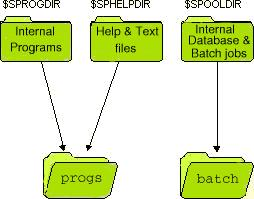
\includegraphics[width=15.131cm,height=10.104cm]{img/diag1.jpg} 

These directories may be relocated by assignment to the three environment variables:
\filename{SPROGDIR}, \filename{SPHELPDIR} and \filename{SPOOLDIR}. These environment variable assignments may be placed in the master
configuration file, \masterconfig, to ensure consistency. The default directories are as follows:

\begin{tabular}{|l | l | l |}
\hline
\bfseries Default location &
\bfseries Environment variable &
\bfseries Function\\\hline
\spooldir &
\filename{SPOOLDIR} &
Jobs and other internal data.\\\hline
\progsdir &
\filename{SPROGDIR} &
Internal programs\\\hline
\progsdir &
\filename{SPHELPDIR} &
Global help and message files\\\hline
\end{tabular}

Take care not to assign values to these environment variables
arbitrarily; very strange things will happen if one part of \ProductName{} is
using one set of directories and some other part is using another!

\section{IPC Facilities}
\ProductName{} uses the ``System V IPC facilities'' to communicate with itself internally.

\begin{itemize}
\item One message queue is used to send requests for the main scheduler process, \progname{btsched}.
\item One shared memory segment saves jobs on the queue. This is periodically written out to the file \filename{btsched\_jfile}
in the spool directory.
\item One shared memory segment saves variables. This is likewise periodically written out to the file \filename{btsched\_vfile}.
\item One shared memory segment is used to buffer pending requests as the size of messages which may be sent on message queues is limited on many systems.
\item One set of semaphores controls access to the shared memory segments.
\item One set of semaphores is used for network locking.
\end{itemize}
The IPC facilities can be displayed by running \progname{ipcs}. The items in question are owned by \batchuser{}
with a key of \exampletext{0x5869Bxxx}.

The system utility \PrXbRipc{} provided in the installation directory may be used to inspect the IPC facilities
especially after a crash and optionally to delete them.

The shared memory used for jobs and variables may have to be reallocated if the number of jobs or variables exceeds the initial amount
allocated. On some systems this may be difficult if other software is in use which has exhausted the available shared memory space. If there are difficulties in this area, make sure to start \ProductName{} with a reservation of the appropriate amount of space. See the
description of \PrBtstart.

On some versions of \ProductName{} these shared memory segments may be replaced by memory-mapped files. On releases of
\ProductName{} subsequent to November 2004, file locks are usually used instead of semaphores.

\section{Files used by \ProductName{}}
The following sections list the files used and created by \ProductName{}.

\subsection{Internal spool files}
The following \ProductName{} internal files are held in the spool directory, which by default is \spooldir:

\begin{tabular}{|l|p{12cm}|}\hline
\bfseries File &
\bfseries Purpose\\\hline
\exampletext{btufile6} &
User permissions (the ``6'' denotes
the ``major'' release).\\\hline
\exampletext{btcharges6} &
User charges (the ``6'' denotes the
``major'' release)
\textbf{deprecated}\\\hline
\exampletext{cifile} &
Specification of command interpreters\\\hline
\exampletext{holfile} &
Days set to be holidays\\\hline
\exampletext{btsched\_jfile} &
Saved record of jobs\\\hline
\exampletext{btsched\_vfile} &
Saved record of variables\\\hline
\exampletext{btsched\_reps} &
Report file holding any messages output by
\progname{btsched}\\\hline
\exampletext{SPnnnnnnnn} &
Queued jobs\\\hline
\exampletext{SOnnnnnnnn} &
Standard output of pending jobs\\\hline
\exampletext{ERnnnnnnnn} &
Standard error of pending jobs\\\hline
\exampletext{NTnnnnnnnn} &
Local copy of remote job\\\hline
\exampletext{btmm\_jobs} &
\textit{If using memory-mapped files rather than shared memory} live memory-mapped file of job queue.\\\hline
\exampletext{btmm\_vars} &
\textit{If using memory-mapped files rather than shared memory} live memory-mapped file of variables.\\\hline
\exampletext{btmm\_xfer} &
\textit{If using memory-mapped files rather than shared memory} live memory-mapped buffer file.\\\hline
\end{tabular}

The above files are owned by \batchuser. Unused copies of
the last four kinds of files may safely be deleted. The nnnnnnnn
component of the file name is derived from the batch job number.

Please note in particular the file \filename{btsched\_reps}.
This is the system log file and processes such as \progname{btsched} and \progname{xbnetserv}
send messages to it in the event of error conditions arising. If you have any support questions, please look in this file.

\subsection{Help and Message files}
\IfXi{In common with other Xi Software products, }\ProductName{} reads all of its messages from a series of text files (apart from the
``\exampletext{help I cannot find the message file}'' messages). The user may adjust these to tailor the
command interface, help and error messages to be suitable for the particular installation. These are \textit{system-wide} message files.
It is also possible to set up customised versions for individual users or applications.

The following files are, by default, owned by \batchuser{} and held in the directory \progsdir.

\begin{tabular}{|l|l|}
\hline
\bfseries File &
\bfseries Purpose\\\hline
\filename{btq.help} &
Screen layout, messages and key assignments for
\PrBtq\\\hline
\filename{btuser.help} &
Screen layout, messages and key assignments for
\PrBtuser\\\hline
\filename{btrest.help} &
Messages and arguments for other user programs\\\hline
\filename{btint-config} &
Message file for \progname{btsched},
\progname{btwrite} and
\progname{xbnetserv}\\\hline
\filename{filemon.help} &
Messages for file monitor option
\progname{btfilemon}\\\hline
\filename{xmbtq.help} &
Job and Variable list specifications for
\PrXbtq{} and \PrXmbtq\\\hline
\filename{xmbtr.help} &
Job and Variable list specifications for
\PrXbtr{} and \PrXmbtr\\\hline
\filename{xmbtuser.help} &
Job and Variable list specifications for
\PrXbtuser{} and \PrXmbtuser\\\hline
\end{tabular}

Refer to the chapters on Configuration and Extensions of both the System Reference Manual and this Administration Guide for details of
how to modify these files as may be required.

\subsection{Configuration files}
Various programs allow sets of options to be written into local ``configuration files''
\configurationfile{} in the working directory, or a more global \homeconfigpath{} file off the user's home directory
so that further runs of those programs pick up a different selection of options from the defaults.

These are text files containing sets of options for various programs, which may be edited by the user, but are normally edited by the
programs concerned.

\subsection{Configuration files held in \etcname}
The following files are always held in the system directory \filename{\etcname}.

\subsubsection{\manualProduct{} Hosts and Clients File}
The file \hostsfile is used on networked installations of \ProductName{} to denote details of the remote hosts and
clients to which connection is to be made. This is fully described in the System Reference Manual.

\subsubsection{\manualProduct{} Master Configuration File}
In order to work properly, the scheduler process and all the other programs must be started with the same environment variables. For
convenience, the environment may be initialised for each program by creating a master configuration file \masterconfig.

This file contains a list of environment variable assignments. Any environment variables not defined on entry to any of the programs are
initialised from this file. Any environment variables used by \ProductName{} may be included in this file, not just those shown in the example.

For example:

\begin{expara}

SPOOLDIR:/usr1/spool/batch

SPROGDIR:/usr1/spool/bin

MAILER=/usr/lib/sendmail

\end{expara}

An environment variable declared using the equality sign \exampletext{=} will be included in the environment of all
batch jobs that are submitted. This may not be wanted for all variables, in particular the directories pointed to by
\filename{SPOOLDIR}, \filename{SPROGDIR} and \filename{SPHELPDIR}, as if the batch jobs contain these, they
will may be ``exported'' to other machines on the network for which they would be inappropriate. To avoid jobs
inheriting environment variables from the configuration file declare them using the colon.

Please note that the text to the right of the colon or \exampletext{=} sign is taken literally; there is no recursive
expansion of \exampletext{\$name} constructs.

\subsubsection{\ProductName{} Static Environment File}
If there are a lot of environment variables, the common ones may be saved in a static environment file with only the
``differences'' from the file held in the jobs.

This file is saved as \batchenv{} as just environment variable assignments.

Alternative files to \batchenv{} can be specified by including the following line in \masterconfig:

\begin{expara}

BATCHENV:file1,file2....

\end{expara}

These files are read in sequence and constitute the new environment.

\section{Ports and Network Services}
\ProductName{} also uses 7 entries in the services file, \filename{/etc/services}. When installed with the default
values the entries will look like this:

\begin{expara}
\IfXi{
xibatch \ 2050/tcp \ \# Connection port for \manualProduct{}

xibatch \ 2050/udp \ \# Probe port for \manualProduct{}

btq \ \ \ \ \ 2150/tcp \ \# Feeder port for \manualProduct{}

xbnetsrv 2250/tcp \ \# DOS client enqueue port for \manualProduct{}

xbnetsrv 2250/udp \ \# DOS client enquiry port for \manualProduct{}

xbapi \ \ \ 2260/tcp \ \# API access port for \manualProduct{}

xbapi \ \ \ 2260/udp \ \# API monitor port for \manualProduct{}

}
\IfGNU{
gnubatch \ \ \ \ \ \ \ 48104/tcp \# Connection port

gnubatch \ \ \ \ \ \ \ 48104/udp \# Probe port

gnubatch-feeder 48105/tcp \# Feeder port for \manualProduct{}

gnubatch-netsrv 48106/tcp \# External job submission

gnubatch-netsrv 48106/udp \# Client access

gnubatch-api \ \ \ 48107/tcp \# API

gnubatch-api \ \ \ 48107/udp \# API (for wakeup messages)

}
\end{expara}

The port numbers can be changed to avoid clashing with those used by other applications, but
all hosts in a given installation must use the same numbers if \ProductName{} connections are to be made.

\IfXi{Please note the different spelling of the services entry, often limited to 8
characters on some older Unix systems, of \filename{xbnetsrv}, the service, and the program \progname{xbnetserv}.}

The installation script will set up entries for the \ProductName{} TCP \& UDP connections in the \filename{/etc/services} file.

If you are using a name service like NIS instead of the services file, the entries must be copied to that service.

\IfXi{It is possible that the port/socket numbers used as standard by \ProductName{} will conflict with another product.
If this is the case they can be moved by editing the \filename{/etc/services} file after installation. The entries are normally in the 2000 to 2300 range, if you move them it is simplest to add one or more thousand to each entry.

For example, if there are no other entries between 5000 and 6000 the standard could be changed to:

\begin{expara}

xibatch \ \textbf{5}050/tcp \ \# Connection port for \manualProduct{}

xibatch \ \textbf{5}050/udp \ \# Probe port for \manualProduct{}

btq \ \ \ \ \ \textbf{5}150/tcp \ \# Feeder port for \manualProduct{}

xbnetsrv \textbf{5}250/tcp \ \# DOS client enqueue port for \manualProduct{}

xbnetsrv \textbf{5}250/udp \ \# DOS client enquiry port for \manualProduct{}

xbapi \ \ \ \textbf{5}260/tcp \ \# API access port for \manualProduct{}

xbapi \ \ \ \textbf{5}260/udp \ \# API monitor port for \manualProduct

\end{expara}
}


